\documentclass[a4,12pt]{seminar}

\usepackage{talk}
\newpsstyle{circle}{linewidth=0.2pt, linestyle=solid, linecolor=black, fillcolor=cyan, fillstyle=solid}
\newpsstyle{arrow}{arrowsize=2mm,linewidth=0.5pt, linestyle=solid, linecolor=black}
\newpsstyle{arrowg}{arrowsize=2mm,linewidth=0.5pt, linestyle=solid, linecolor=gray}

\def\alabel#1#2#3{\rnode{#2}{\psframebox[linewidth=0.2pt, linestyle=solid, framearc=0.5, fillstyle=solid, fillcolor=#3]{\footnotesize #1}}}
\def\ylabel#1#2{\alabel{#1}{#2}{yellow}}
\def\glabel#1#2{\alabel{#1}{#2}{green}}

%%%%%%%%%%%%%%%%%%%%%%%%%%%%%%%%%%%%%%%%%%%%%%%
%%%%%%%%%%%%%%%%%%%%%%%%%%%%%%%%%%%%%%%%%%%%%%%

\def\allinterface{%
\psset{unit=1.25mm}
%
\rput(-32,-6){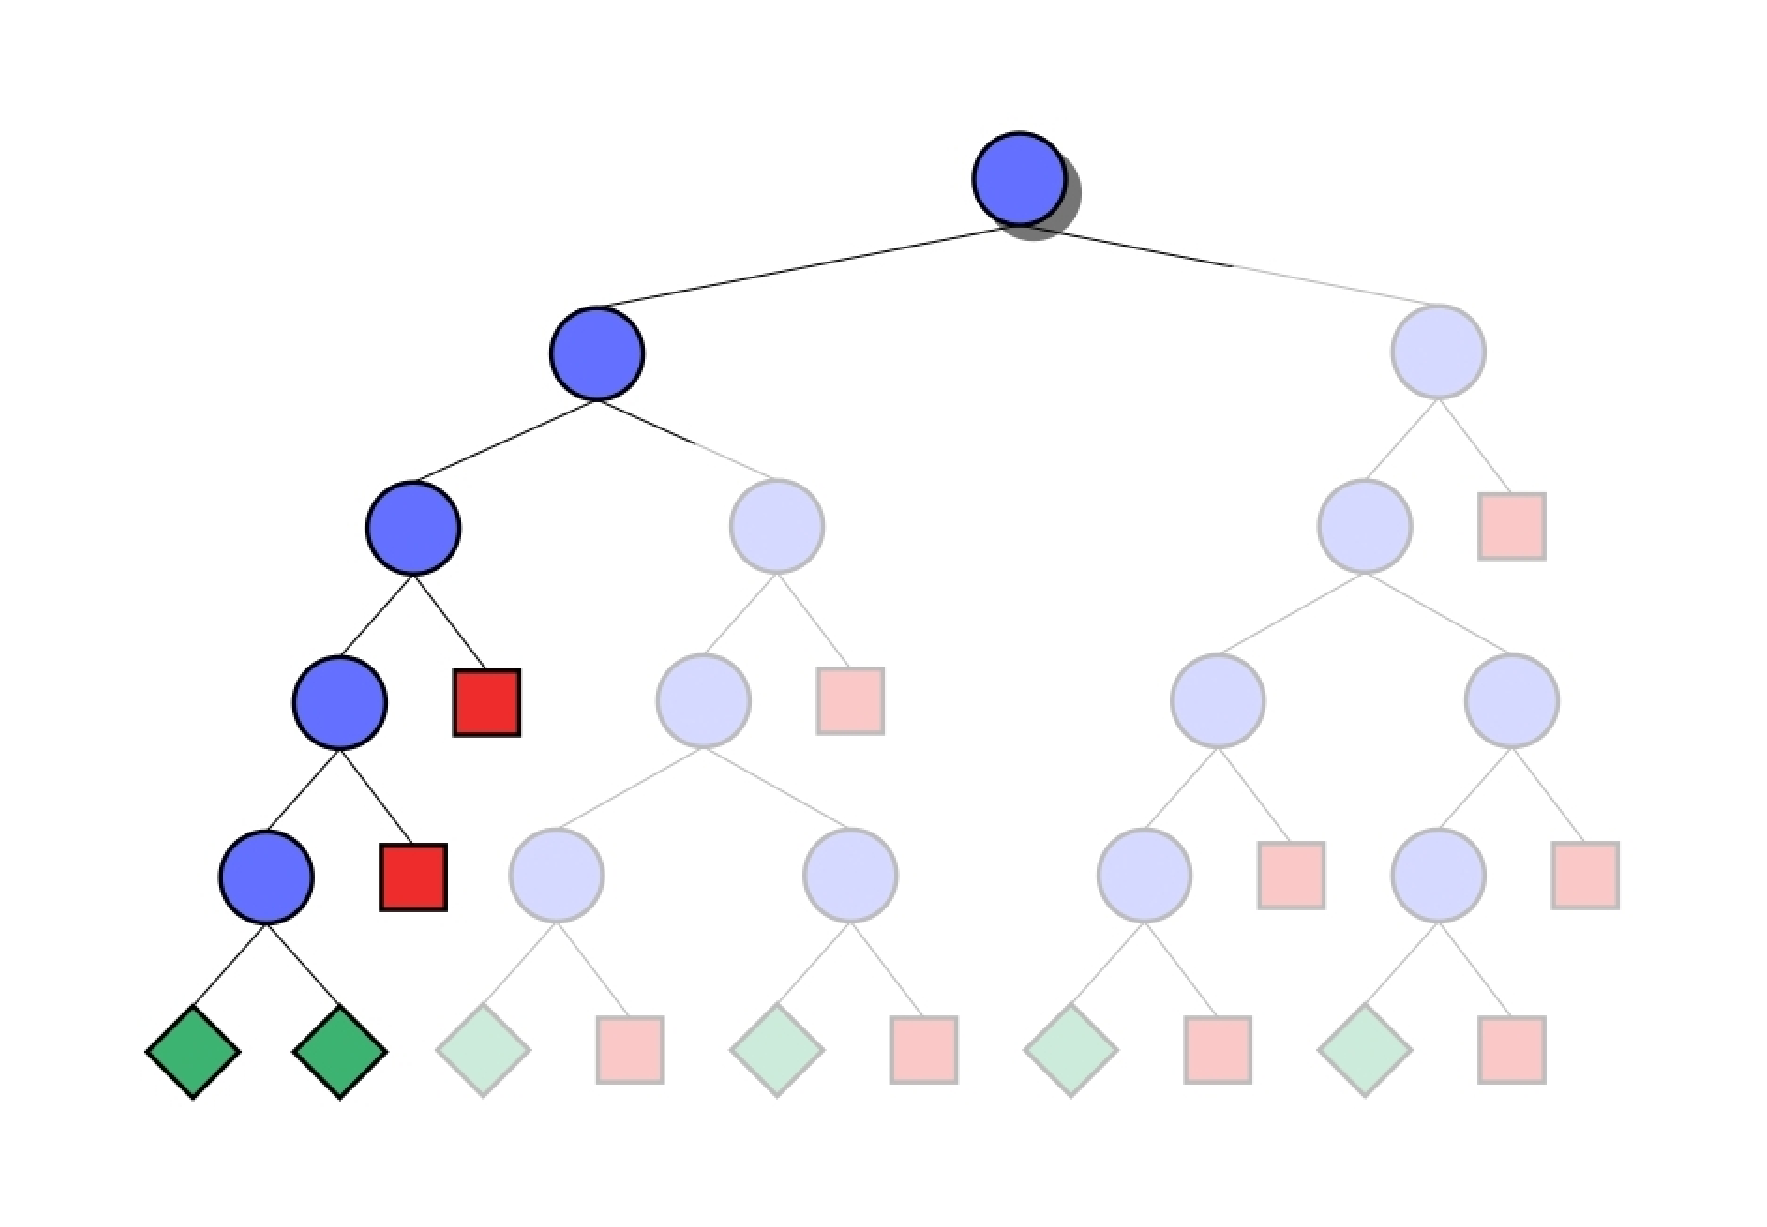
\includegraphics[height=24mm]{part1.eps}}
\rput(18,-21){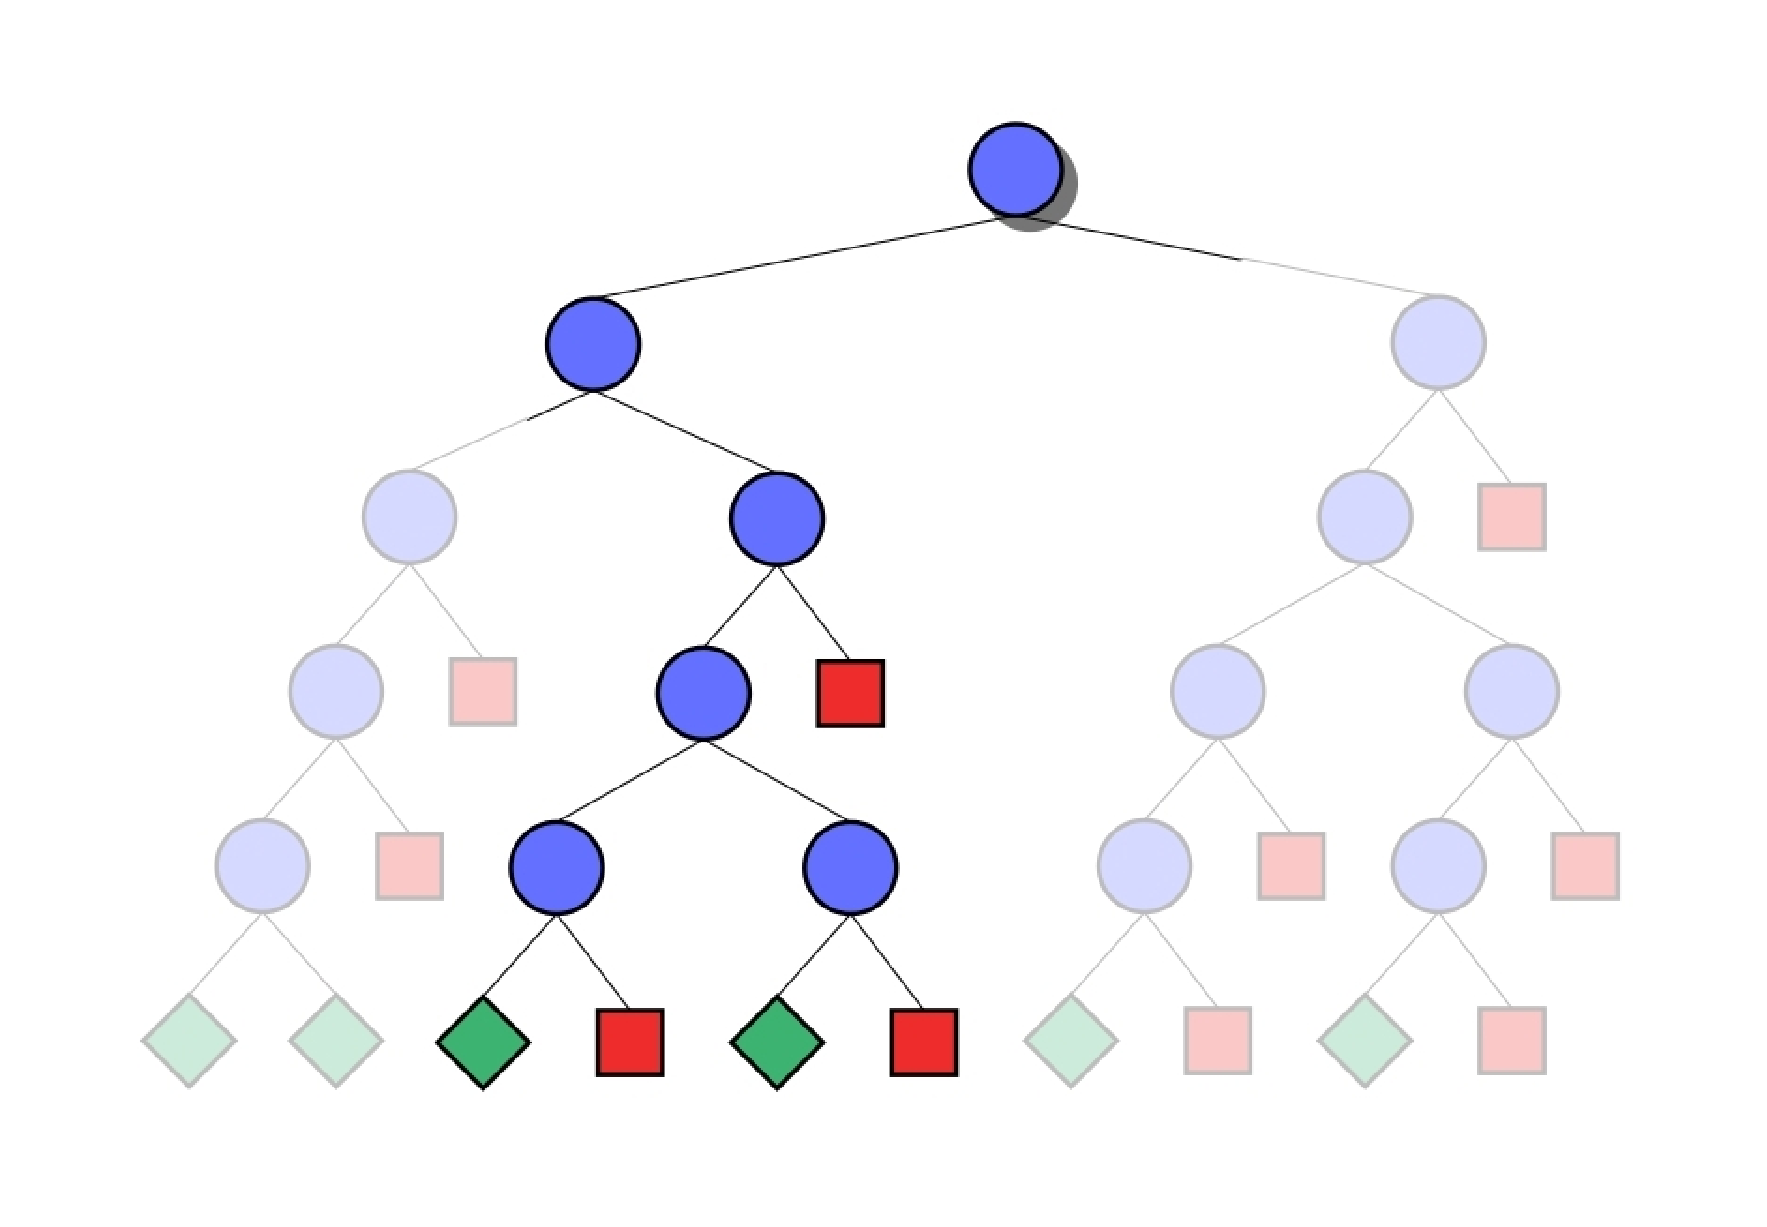
\includegraphics[height=24mm]{part2.eps}}
\rput(30,0){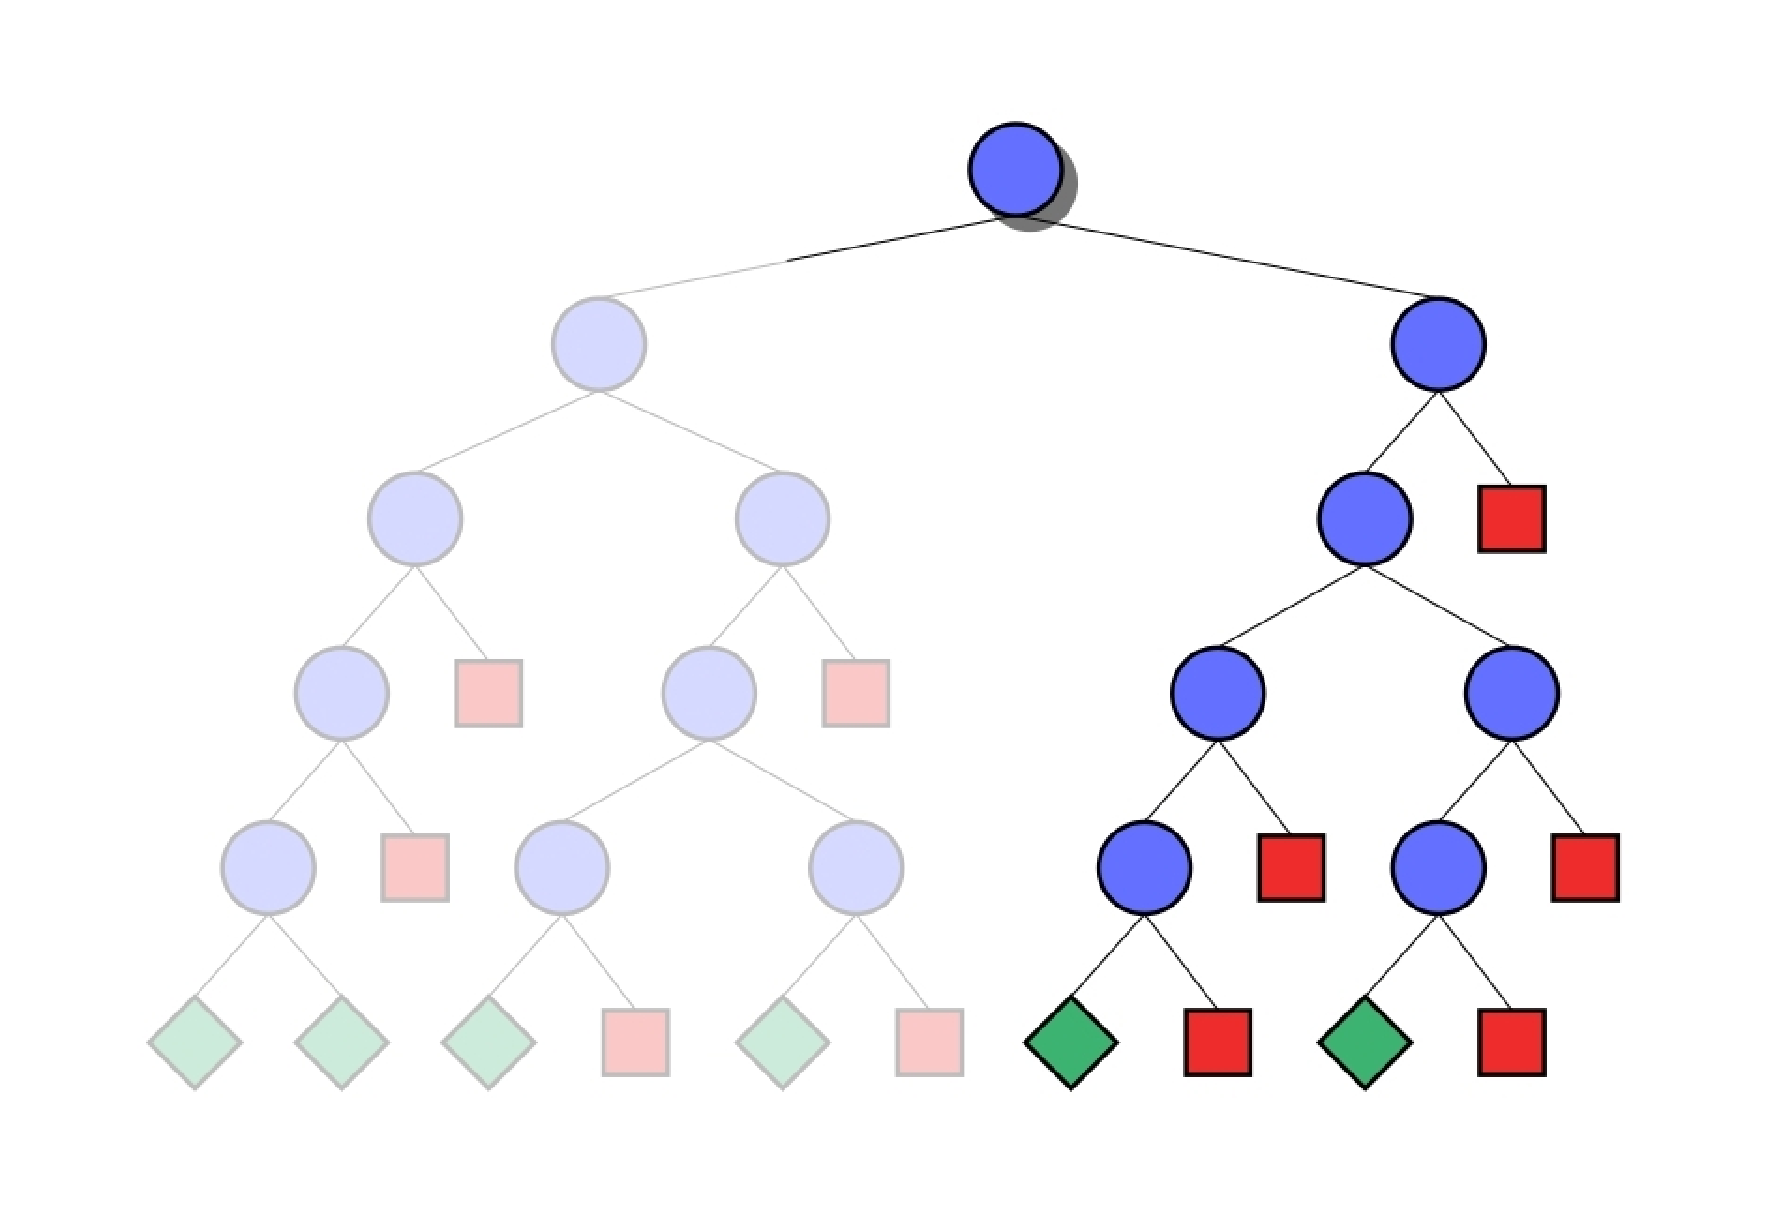
\includegraphics[height=24mm]{part3.eps}}
%
\cnodeput[style=circle](0,0){manager}{Manager}
\cnodeput[style=circle](20,-10){worker1}{w}
\cnodeput[style=circle](-30,5){worker2}{w}
\cnodeput[style=circle](30,10){worker3}{w}
\cnodeput[style=circle](-5,20){worker4}{w}
%
\ncline[style=arrow,doubleline=true]{<|-|>}{worker1}{manager}
\ncline[style=arrow,doubleline=true]{<|-|>}{worker2}{manager}
\ncline[style=arrow,doubleline=true]{<|-|>}{worker3}{manager}
\ncline[style=arrow,doubleline=true]{<|-|>}{worker4}{manager}
%
\rput(10,20){Workers}
%
}

%%%%%%%%%%%%%%%%%%%%%%%%%%%%%%%%%%%%%%%%%%%%%%%
%%%%%%%%%%%%%%%%%%%%%%%%%%%%%%%%%%%%%%%%%%%%%%%

\def\interfaceA{%
\psset{unit=1.25mm}
%
\cnode[style=circle](-45,-15){5}{worker}
\cnode[style=circle](0,-15){5}{manager}
%
\rput(0,-25){Manager}
\rput(-45,-25){Worker}
%
\rput(-22,-5){\ylabel{register}{register}}
\ncline[style=arrow]{-}{worker}{register}
\ncline[style=arrow]{-|>}{register}{manager}
%
\rput(-22,-15){\glabel{find}{find}}
\ncline[style=arrow]{-}{worker}{find}
\ncline[style=arrow]{-|>}{find}{manager}
%
\rput(-22,-25){\glabel{collect}{collect}}
\ncline[style=arrow]{-}{worker}{collect}
\ncline[style=arrow]{-|>}{collect}{manager}
}

\def\interfaceB{%
\psset{unit=1.25mm}
%
\cnode[style=circle](-45,-15){5}{worker}
\cnode[style=circle](0,-15){5}{manager}
%
\rput(0,-25){Manager}
\rput(-45,-25){Worker}
%
\rput(-22,-5){\glabel{share}{share}}
\ncline[style=arrow]{<|-}{worker}{share}
\ncline[style=arrow]{-}{share}{manager}
%
\rput(-22,-15){\glabel{explore}{explore}}
\ncline[style=arrow]{<|-}{worker}{explore}
\ncline[style=arrow]{-}{explore}{manager}
%
\rput(-22,-25){\ylabel{stop}{stop}}
\ncline[style=arrow]{<|-}{worker}{stop}
\ncline[style=arrow]{-}{stop}{manager}
}


%%%%%%%%%%%%%%%%%%%%%%%%%%%%%%%%%%%%%%
%%%%%%%%%%%%%%%%%%%%%%%%%%%%%%%%%%%%%%
%%%%%%%%%%%%%%%%%%%%%%%%%%%%%%%%%%%%%%
%%%%%%%%%%%%%%%%%%%%%%%%%%%%%%%%%%%%%%
%%%%%%%%%%%%%%%%%%%%%%%%%%%%%%%%%%%%%%

\def\interface{%
\psset{unit=1mm}
%
\cnode[style=circle](-22,-15){5}{manager}
\cnode[style=circle](22,-15){5}{worker}
%
\rput(-22,3){Manager}
\rput(22,3){Worker}
%
%%%%%%%%%%%%%%%%%%%%%%%%%%%%%%%%%%%%%
%
\rput(-40,0){\ylabel{register}{register}}
\ncline[style=arrow]{-|>}{register}{manager}
%
\rput(-50,-10){\glabel{find}{find}}
\ncline[style=arrow]{-|>}{find}{manager}
%
\rput(-50,-20){\glabel{collect}{collect}}
\ncline[style=arrow]{-|>}{collect}{manager}
%
\rput(-40,-30){\ylabel{log}{log}}
\ncline[style=arrow]{-|>}{log}{manager}
%
%%%%%%%%%%%%%%%%%%%%%%%%%%%%%%%%%%%%%
%
\rput(0,-5){\glabel{share}{share}}
\ncline[style=arrowg]{-|>}{manager}{share}
\ncline[style=arrow]{-|>}{share}{worker}
%
\rput(0,-15){\glabel{explore}{explore}}
\ncline[style=arrowg]{-|>}{manager}{explore}
\ncline[style=arrow]{-|>}{explore}{worker}
%
\rput(0,-25){\ylabel{stop}{stop}}
\ncline[style=arrowg]{-|>}{manager}{stop}
\ncline[style=arrow]{-|>}{stop}{worker}
%
%%%%%%%%%%%%%%%%%%%%%%%%%%%%%%%%%%%%%%
%
\rput(45,0){\ylabel{register}{register2}}
\ncline[style=arrowg]{-|>}{worker}{register2}
%
\rput(45,-10){\glabel{find}{find2}}
\ncline[style=arrowg]{-|>}{worker}{find2}
%
\rput(45,-20){\glabel{collect}{collect2}}
\ncline[style=arrowg]{-|>}{worker}{collect2}
%
\rput(45,-30){\ylabel{log}{log2}}
\ncline[style=arrowg]{-|>}{worker}{log2}
%
}


\begin{document}
\pagestyle{fancy}


%%%%%%%%%%%%%%%%%%%%%%%%%%%%%%%%%%%%%%%%%%%%%%%%%%%%%%%%%%%
%%             First PAGE
%%%%%%%%%%%%%%%%%%%%%%%%%%%%%%%%%%%%%%%%%%%%%%%%%%%%%%%%%%%
\begin{slide}
\Title{A distributed search engine}
\begin{center}
\rput(0,-30mm){\allinterface}
\end{center}
\end{slide}


%%%%%%%%%%%%%%%%%%%%%%%%%%%%%%%%%%%%%%%%%%%%%%%%%%%%%%%%%%%
%%      The INTERFACES
%%%%%%%%%%%%%%%%%%%%%%%%%%%%%%%%%%%%%%%%%%%%%%%%%%%%%%%%%%%
\begin{slide}
\Title{Interfaces}
\begin{flushright}
\rput(-6mm,14mm){\interfaceA}
%%
\begin{minipage}{0.45\linewidth}
\scriptsize
\vskip 8mm
\begin{alltt}
type \ttv manager\_intf =
    \{\ylab{register}: \ttv worker\_intf \tar unit ,
     \glab{find    }: \hphantom{\ttv}        unit \tar unit ,
     \glab{collect }:             \ttv \tar unit \}
\end{alltt}
\end{minipage}
\hspace{2mm}

\vskip 14mm

\rput(-6mm,10mm){\interfaceB}
%%
\begin{minipage}{0.45\linewidth}
\scriptsize
\vskip 4mm
\begin{alltt}
type \ttv worker\_intf =
    \{\glab{share  }:  \hphantom{\ttv}unit \tar (\ttv work) option,
     \glab{explore}: \ttv work \tar unit ,
     \ylab{stop   }: \hphantom{\ttv} unit \tar unit \}
\end{alltt}
\end{minipage}
\hspace{2mm}

\end{flushright}
\end{slide}




%%%%%%%%%%%%%%%%%%%%%%%%%%%%%%%%%%%%%%%%%%%%%%%%%%%%%%%%%%%
%%      Manager IMPLEMENTATION
%%%%%%%%%%%%%%%%%%%%%%%%%%%%%%%%%%%%%%%%%%%%%%%%%%%%%%%%%%%
\begin{slide}
\Title{Manager Implementation}
\vskip 6mm

\begin{alltt}
\footnotesize
\kwd{fun} \blab{register} workerIntf = \cldots
\kwd{fun} \blab{find}     ()         = \cldots
\kwd{fun} \blab{collect}  sol        = \cldots

\iftrue
\kwd{val} \Blab{remoteRegister} = \cdi{Remote.proxy} \blab{register}
\kwd{val} \Blab{remoteFind}     = \cdi{Remote.proxy} \blab{find}
\kwd{val} \Blab{remoteCollect}  = \cdi{Remote.proxy} \blab{collect}


\kwd{val} managerInterface =
  \kwd{\{}\ylab{register} = \Blab{remoteRegister} ,
   \glab{find}     = \Blab{remoteFind} ,    
   \glab{collect}  = \kwd{fn} args \kwd{=>} \cdi{spawn} (\Blab{remoteCollect} args)\kwd{\}} \comt{(Asynchronous)}
\else
\kwd{val} managerInterface =
  \kwd{let} \kwd{val} \Blab{register} = \cdi{Remote.proxy} \blab{register}
      \kwd{val} \Blab{find}     = \cdi{Remote.proxy} \blab{find}
      \kwd{val} \Blab{collect}  = \cdi{Remote.proxy} \blab{collect}
  \kwd{in}

  \kwd{\{}\ylab{register} = \Blab{register} ,
   \glab{find}     = \Blab{find} ,    
   \glab{collect}  = \kwd{fn} args \kwd{=>} \cdi{spawn} (\Blab{collect} args)\} \comt{(Asynchronous)}

  \kwd{end}
\fi
\end{alltt}
%
\vskip -80mm
\rput(110mm,-4mm){\blab{\normalsize Definitions}}
\rput(110mm,-26mm){\Blab{\normalsize Remote functions}}
\rput(110mm,-31.75mm){\Blab{\normalsize (RPC)}}
\rput(110mm,-52mm){\glab{\normalsize Export}}
\rput(110mm,-56.5mm){\glab{\normalsize Interface}}
%
\end{slide}


%%%%%%%%%%%%%%%%%%%%%%%%%%%%%%%%%%%%%%%%%%%%%%%%%%%%%%%%%%%
%%           Distribution
%%%%%%%%%%%%%%%%%%%%%%%%%%%%%%%%%%%%%%%%%%%%%%%%%%%%%%%%%%%
\begin{slide}
\Title{Distribution}

\begin{alltt}
\footnotesize
\kwd{val} \Blab{parcel} = \cdi{pack} (\kwd{val} interface = managerInterface)
                \cdi{:>} \,\,(\kwd{val} interface : (int vector) manager_interface)
\kwd{val} \Blab{url}    = \cdi{Remote.offer} \Blab{parcel}
\end{alltt}

\vskip 10mm

\begin{dinglist}{\dingA}
\item \cdi{\texttt{Remote.offer}} starts a http server which ``offers'' the manager interface.

\item We send the \Blab{\normalsize \texttt{url}} by ssh
\end{dinglist}

\begin{alltt}
OS.Process.system \textcolor{blue}{"ssh -f \textit{host} alicerun Worker \Blab{url}"}
\end{alltt}

\end{slide}



%%%%%%%%%%%%%%%%%%%%%%%%%%%%%%%%%%%%%%%%%%%%%%%%%%%%%%%%%%%
%%           Worker
%%%%%%%%%%%%%%%%%%%%%%%%%%%%%%%%%%%%%%%%%%%%%%%%%%%%%%%%%%%
\begin{slide}
\Title{Workers}

\begin{alltt}
\footnotesize
\comt{(* Get and unpack the parcel. *)}
\kwd{structure} \Blab{Parcel} =
         \cdi{unpack} (\cdi{Remote.take} \Blab{url})
           \cdi{:} \,\,(\kwd{val} interface : (int vector) manager_interface)

\comt{(* Get functions from the manager interface. *)}
\kwd{val} managerIntf = \Blab{Parcel}.interface
\kwd{val} \ylab{register}    = #{register} managerIntf
\kwd{val} \glab{find}        = #{find} managerIntf
\kwd{val} \glab{collect}     = #{collect} managerIntf

\comt{(* Each function call automatically uses the remote implementation. *)}
\ldots find () \ldots
\ldots collect solution \ldots
\end{alltt}
\end{slide}

\begin{slide}
\Title{Conclusion}

\vskip 4mm
Distribution and concurrency are achieved using only
a few well-defined \boite{primitives}
\vskip 8mm

\begin{dinglist}{\dingC}
\item \cdi{\texttt{Remote.proxy}}, \cdi{\texttt{Remote.offer}} and \cdi{\texttt{Remote.take}}
\item \cdi{\texttt{pack}} and \cdi{\texttt{unpack}}
\item \cdi{\texttt{spawn}}
\end{dinglist}

\vskip 5mm
Static type-checking makes the use of these primitives \boite{safe}
with respect to types.

\end{slide}

\end{document}
